\documentclass[11pt]{article}
\usepackage[a4paper]{geometry}
\usepackage{polski}
\usepackage[utf8]{inputenc}
\usepackage{hyperref}
\usepackage[table,xcdraw]{xcolor}
\definecolor{mygray}{gray}{0.5}
\usepackage{graphicx}
\usepackage{forest}
\usepackage[T1]{fontenc}

\tikzset{
  block/.style={
    rectangle,
    draw=black,
    fill=gray!10,
    rounded corners,
    text centered,
    minimum width=3cm,
    minimum height=1cm
  },
  arrow/.style={
    thick,
    ->,
    >=Stealth
  }
}
\usepackage{float}
\usepackage{adjustbox}
\usepackage[usestackEOL]{stackengine} 
\usepackage{caption}
\usetikzlibrary{shapes,arrows,chains}
\usetikzlibrary{calc}
\linespread{1.3}
\usepackage{listings}
\usepackage{indentfirst}
\usepackage{amsmath}
\usepackage{amssymb}
\usepackage{enumitem}
\usepackage{multirow}
\usepackage{multicol}
\usepackage{array}
\usepackage{subcaption}
\usepackage{tabularx}
\usepackage{makecell}
\usepackage{longtable}
\renewcommand{\arraystretch}{1.4}
\usepackage{tikz}
\usetikzlibrary{arrows.meta, positioning, trees, mindmap}
\usepackage{lscape}
\usepackage{booktabs}
\usepackage{colortbl}
\usepackage{pdfpages}

\geometry{a4paper, margin=1in}

\lstset{
  backgroundcolor=\color{white},   
  basicstyle=\ttfamily\footnotesize,
  breaklines=true,                 
  frame=single,                    
  keywordstyle=\color{blue},       
  language=Python,                 
  numbers=left,                    
  numberstyle=\tiny\color{mygray}, 
  rulecolor=\color{black},         
  tabsize=2,
  extendedchars=true,
  inputencoding=utf8,
  literate={ą}{{\k{a}}}1 {ć}{{\'c}}1 {ę}{{\k{e}}}1 {ł}{{\l{}}}1 {ń}{{\'n}}1 {ó}{{\'o}}1 {ś}{{\'s}}1 {ź}{{\'z}}1 {ż}{{\.z}}1
           {Ą}{{\k{A}}}1 {Ć}{{\'C}}1 {Ę}{{\k{E}}}1 {Ł}{{\L{}}}1 {Ń}{{\'N}}1 {Ó}{{\'O}}1 {Ś}{{\'S}}1 {Ź}{{\'Z}}1 {Ż}{{\.Z}}1
}

\begin{document}

% ============================ STRONA TYTUŁOWA ============================
\begin{titlepage}
\newcommand{\HRule}{\rule{\linewidth}{0.5mm}}
\centering

\includegraphics[scale=0.21]{pwr-logo.png}\\[2cm]

\textsc{\Large Politechnika Wrocławska}\\[0.5cm]
\textsc{\large Wydział Informatyki i Telekomunikacji}\\[0.5cm]
\textsc{\large Kierunek: Informatyka techniczna}\\[0.5cm]
\textsc{\large Specjalność: Systemy informatyki w medycynie}\\[2cm]

\HRule \\[0.4cm]
{\huge \bfseries SymptoCheck}\\[0.4cm]
{\large Projekt aplikacji webowej wykorzystującej API Gemini do analizy objawów chorobowych}\\[0.4cm]
\HRule \\[1cm]

\begin{minipage}[t]{0.45\textwidth}
\flushleft \large
\emph{Autorzy:}\\
Amelia \textsc{Draga} 272866 \\
Artur \textsc{Gierlak} 272957
\end{minipage}
\hfill
\begin{minipage}[t]{0.45\textwidth}
\flushright \large
\emph{Prowadzący:} \\
dr hab. inż. Mariusz \textsc{Topolski}
\end{minipage}

\vfill
\centering
Wrocław, listopad 2025 r.
\end{titlepage}

\newpage
\tableofcontents
\newpage
\listoffigures
\newpage

% ============================ WSTĘP ============================
\section{Wstęp}
W ramach zajęć \textit{Projektowanie systemów informatyki medycznej} należało stworzyć dowolną aplikację o tematyce medycznej. Dodatkowym wymaganiem projektu było zaimplementowanie \textbf{API}, które umożliwia wymianę danych pomiędzy warstwami systemu lub integrację z zewnętrznym serwisem.


\subsection{Cel projektu}
Celem projektu \textbf{SymptoCheck} było stworzenie aplikacji internetowej o tematyce medycznej, wykorzystującej sztuczną inteligencję do wspomagania wstępnej diagnozy na podstawie objawów podanych przez użytkownika. Projekt miał na celu połączenie technologii webowych z dostępem do modelu językowego \textit{Gemini 2.5 Flash} udostępnianego przez API Google. Dzięki temu użytkownik może w prosty sposób uzyskać propozycję potencjalnych diagnoz, prowadzić rozmowę z wirtualnym asystentem oraz przeglądać historię wcześniejszych analiz.
Aplikacja nie zastępuje profesjonalnej konsultacji lekarskiej – jej zadaniem jest jedynie wsparcie informacyjne poprzez analizę opisowych danych o objawach.

\subsection{Opis systemu}
System \textbf{SymptoCheck} został zaprojektowany jako dwuwarstwowa aplikacja webowa składająca się z:
\begin{itemize}
    \item \textbf{frontendu} zbudowanego w technologii \textbf{React (Vite, TailwindCSS)} , odpowiedzialnego za interakcję z użytkownikiem, prezentację wyników oraz czat z asystentem,
    \item \textbf{backendu} opartego na frameworku \textbf{Django REST}, który odpowiada za przetwarzanie żądań, komunikację z \textbf{API modelu Gemini} oraz zapisywanie historii analiz w lokalnej bazie danych \textbf{SQLite}.
\end{itemize}

Głównym celem działania systemu jest umożliwienie użytkownikowi uzyskania wstępnej, poglądowej diagnozy na podstawie opisanych objawów. Dodatkowo aplikacja pozwala na rozmowę z~wirtualnym asystentem medycznym oraz przeglądanie historii wcześniejszych analiz, co zwiększa jej funkcjonalność i praktyczne zastosowanie.


\subsection{Zakres projektu}
W ramach projektu \textbf{SymptoCheck} udało się zrealizować wszystkie główne założenia funkcjonalne oraz techniczne systemu. Prace zostały podzielone na część frontendową i backendową, a następnie połączone w działającą całość komunikującą się poprzez \textbf{REST API}.
Po stronie \textbf{backendu} zrealizowano:
\begin{itemize}
    \item konfigurację środowiska Django wraz z integracją \textit{Django REST Framework},
    \item stworzenie modelu danych \texttt{Analysis}, który zapisuje historię wykonanych analiz (objawy, wynik, data),
    \item implementację trzech głównych endpointów API:
    \begin{itemize}
        \item \texttt{/diagnose} – wysyła opis objawów do modelu \textit{Gemini 2.5 Flash} i zwraca analizę w formacie Markdown,
        \item \texttt{/chat} – umożliwia prowadzenie rozmowy z modelem w kontekście medycznym,
        \item \texttt{/analyses} – pozwala na pobranie zapisanej historii analiz,
    \end{itemize}
    \item integrację z \textbf{Gemini API} przy użyciu oficjalnej biblioteki \texttt{google-generativeai},
    \item obsługę wyjątków i błędów API, takich jak brak połączenia lub nieprawidłowy klucz.
\end{itemize}
Po stronie \textbf{frontendu} wykonano:
\begin{itemize}
    \item zaprojektowanie i zaimplementowanie trzech głównych komponentów:
    \begin{itemize}
        \item \texttt{SymptomForm.jsx} – formularz, w którym użytkownik wpisuje objawy i otrzymuje wynik diagnozy,
        \item \texttt{ChatAssistant.jsx} – moduł czatu, który pozwala prowadzić rozmowę z asystentem AI,
        \item \texttt{HistoryList.jsx} – lista historii poprzednich analiz,
    \end{itemize}
    \item zastosowanie biblioteki \textit{React Markdown} do czytelnego wyświetlania wyników zwróconych przez model,
    \item opracowanie prostego i intuicyjnego interfejsu użytkownika z wykorzystaniem \textit{TailwindCSS},
    \item konfigurację komunikacji z backendem poprzez żądania HTTP metodą \texttt{POST} i \texttt{GET}.
\end{itemize}


W efekcie końcowym powstała w pełni działająca aplikacja, która umożliwia analizę objawów i uzyskanie możliwych diagnoz w oparciu o model AI, prowadzenie rozmowy z inteligentnym asystentem medycznym oraz zapisywanie i przeglądanie historii wcześniejszych analiz.
Projekt został ukończony zgodnie z założeniami i spełnia wszystkie wymagania funkcjonalne określone na początku realizacji.


% ============================ ARCHITEKTURA ============================
\newpage
\subsection{Architektura systemu}

Aplikacja \textbf{SymptoCheck} została zaprojektowana w architekturze dwuwarstwowej, składającej się z części \textbf{frontendowej} oraz \textbf{backendowej}. Obie warstwy komunikują się ze sobą za pomocą interfejsu \textbf{REST API}, co zapewnia prostą i niezawodną wymianę danych między użytkownikiem a serwerem.

\begin{itemize}
    \item \textbf{Frontend} — odpowiada za interfejs użytkownika i obsługę logiki po stronie przeglądarki. Został stworzony przy użyciu technologii \textit{React.js}, w środowisku \textit{Vite}, z wykorzystaniem frameworka \textit{TailwindCSS} do stylizacji. Użytkownik wprowadza dane (objawy) w formularzu, a aplikacja przesyła je do serwera w formacie JSON. Wyniki analizy są następnie prezentowane w przejrzystej formie.
    
    \item \textbf{Backend} — pełni rolę warstwy serwerowej i został stworzony w \textit{Django REST Framework}. Jego zadaniem jest przyjmowanie żądań z frontendu, komunikacja z zewnętrznym API modelu \textit{Gemini 2.5 Flash} oraz zwracanie przetworzonych wyników do interfejsu użytkownika. Backend przechowuje również historię analiz w lokalnej bazie danych \textit{SQLite}.
\end{itemize}

Komunikacja pomiędzy frontendem a backendem odbywa się z wykorzystaniem metod \texttt{POST} i \texttt{GET}. Frontend przesyła zapytanie z opisem objawów na odpowiedni endpoint API, a backend wysyła dane do modelu \textit{Gemini 2.5 Flash}, który generuje analizę w formacie tekstowym (Markdown). Następnie wynik jest przekazywany z powrotem do użytkownika i zapisywany w historii.

\begin{figure}[H]
\centering
\begin{tikzpicture}[node distance=2.2cm and 2.6cm, >=Stealth, thick]
% --- first row ---
\node (user) [draw, rounded corners, fill=blue!10, minimum width=2.8cm, minimum height=1cm, text centered] {Użytkownik};
\node (frontend) [draw, rounded corners, fill=green!10, right=of user, minimum width=3cm, minimum height=1cm, text centered] {Frontend (React)};

% --- second row ---
\node (backend) [draw, rounded corners, fill=yellow!10, below=of frontend, minimum width=3cm, minimum height=1cm, text centered] {Backend (Django)};
\node (api) [draw, rounded corners, fill=red!10, right=of backend, minimum width=3cm, minimum height=1cm, text centered] {Gemini API};

% --- arrows ---
\draw[->] (user) -- node[above]{1. Wprowadzenie objawów} (frontend);
\draw[->] (frontend) -- node[right]{2. Zapytanie HTTP} (backend);
\draw[->] (backend) -- node[above]{3. Żądanie do API Gemini} (api);
\draw[<-] (backend) -- node[below]{4. Odpowiedź modelu} (api);
\draw[<-] (frontend) -- node[left]{5. Wynik analizy} (backend);
\draw[<-] (user) -- node[below]{6. Prezentacja wyników} (frontend);

\end{tikzpicture}
\caption{Schemat przepływu danych w architekturze systemu SymptoCheck.}
\end{figure}



Każda z warstw systemu działa niezależnie, co umożliwia łatwe modyfikacje oraz rozwijanie projektu w przyszłości. Na przykład możliwe jest wdrożenie backendu w chmurze, a frontendu jako aplikacji PWA (Progressive Web App). Taka struktura zapewnia także lepszą skalowalność i elastyczność w dalszym rozwoju systemu.

Podsumowując, architektura \textbf{SymptoCheck} opiera się na prostym, ale skutecznym połączeniu Reacta po stronie klienta i Django REST po stronie serwera, z wykorzystaniem API \textit{Gemini 2.5 Flash} jako zewnętrznego źródła inteligentnej analizy.


% ============================ IMPLEMENTACJA BACKENDU ============================
\newpage
\section{Implementacja backendu}

\subsection{Struktura projektu Django}
Backend został zorganizowany zgodnie z konwencją Django. Główne komponenty:
\begin{itemize}
    \item \texttt{backend/} -- folder główny projektu Django z plikami konfiguracyjnymi (\texttt{settings.py}, \texttt{urls.py}),
    \item \texttt{core/} -- aplikacja Django zawierająca logikę biznesową, modele, widoki i endpointy API,
    \item \texttt{manage.py} -- skrypt do zarządzania projektem (migracje, uruchamianie serwera, testy).
\end{itemize}

\subsection{Model danych}
W bazie danych SQLite zdefiniowano model \texttt{Analysis}, który przechowuje historię analiz użytkownika:

\begin{lstlisting}[language=Python]
from django.db import models

class Analysis(models.Model):
    created_at = models.DateTimeField(auto_now_add=True)
    symptoms = models.TextField()
    result_md = models.TextField()  # wynik w formacie Markdown
    confidence_json = models.JSONField(null=True, blank=True)
    
    def __str__(self):
        return f"Analysis #{self.id} @ {self.created_at:%Y-%m-%d %H:%M}"
\end{lstlisting}

Pola modelu:
\begin{itemize}
    \item \texttt{created\_at} -- data i czas utworzenia analizy (ustawiana automatycznie),
    \item \texttt{symptoms} -- tekst wprowadzony przez użytkownika opisujący objawy,
    \item \texttt{result\_md} -- wynik analizy zwrócony przez model AI w formacie Markdown,
    \item \texttt{confidence\_json} -- opcjonalne dane JSON zawierające prawdopodobieństwa poszczególnych diagnoz.
\end{itemize}

\subsubsection{Schemat bazy danych}
Poniższy diagram przedstawia strukturę tabeli \texttt{Analysis} w bazie SQLite:

\begin{figure}[H]
\centering
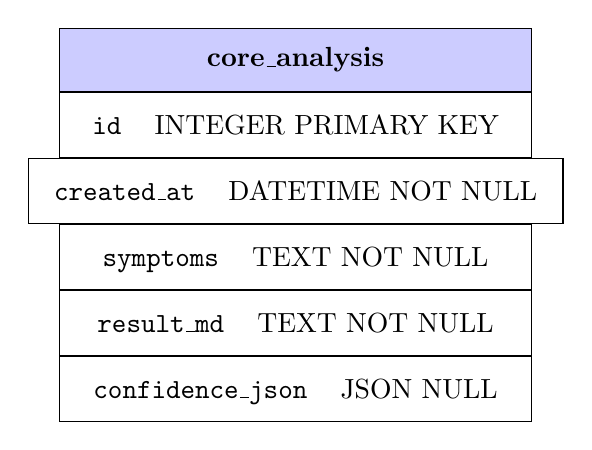
\begin{tikzpicture}[node distance=0.5cm]
  \node[draw, rectangle, minimum width=6cm, minimum height=0.8cm, fill=blue!20] (header) {\textbf{core\_analysis}};
  
  \node[draw, rectangle, minimum width=6cm, anchor=north] (id) at (header.south) {
    \begin{tabular}{l l}
    \texttt{id} & INTEGER PRIMARY KEY
    \end{tabular}
  };
  
  \node[draw, rectangle, minimum width=6cm, anchor=north] (created) at (id.south) {
    \begin{tabular}{l l}
    \texttt{created\_at} & DATETIME NOT NULL
    \end{tabular}
  };
  
  \node[draw, rectangle, minimum width=6cm, anchor=north] (symptoms) at (created.south) {
    \begin{tabular}{l l}
    \texttt{symptoms} & TEXT NOT NULL
    \end{tabular}
  };
  
  \node[draw, rectangle, minimum width=6cm, anchor=north] (result) at (symptoms.south) {
    \begin{tabular}{l l}
    \texttt{result\_md} & TEXT NOT NULL
    \end{tabular}
  };
  
  \node[draw, rectangle, minimum width=6cm, anchor=north] (confidence) at (result.south) {
    \begin{tabular}{l l}
    \texttt{confidence\_json} & JSON NULL
    \end{tabular}
  };
\end{tikzpicture}
\caption{Schemat tabeli \texttt{core\_analysis} w bazie danych SQLite}
\end{figure}

Django automatycznie tworzy tabelę na podstawie modelu podczas wykonania migracji (\texttt{python manage.py migrate}). Nazwa tabeli ma prefiks \texttt{core\_} pochodzący od nazwy aplikacji Django.

\subsection{Szczegółowy przepływ danych dla analizy objawów}
Poniższy diagram sekwencji ilustruje dokładny przepływ danych podczas wykonywania analizy objawów:

\begin{figure}[H]
\centering
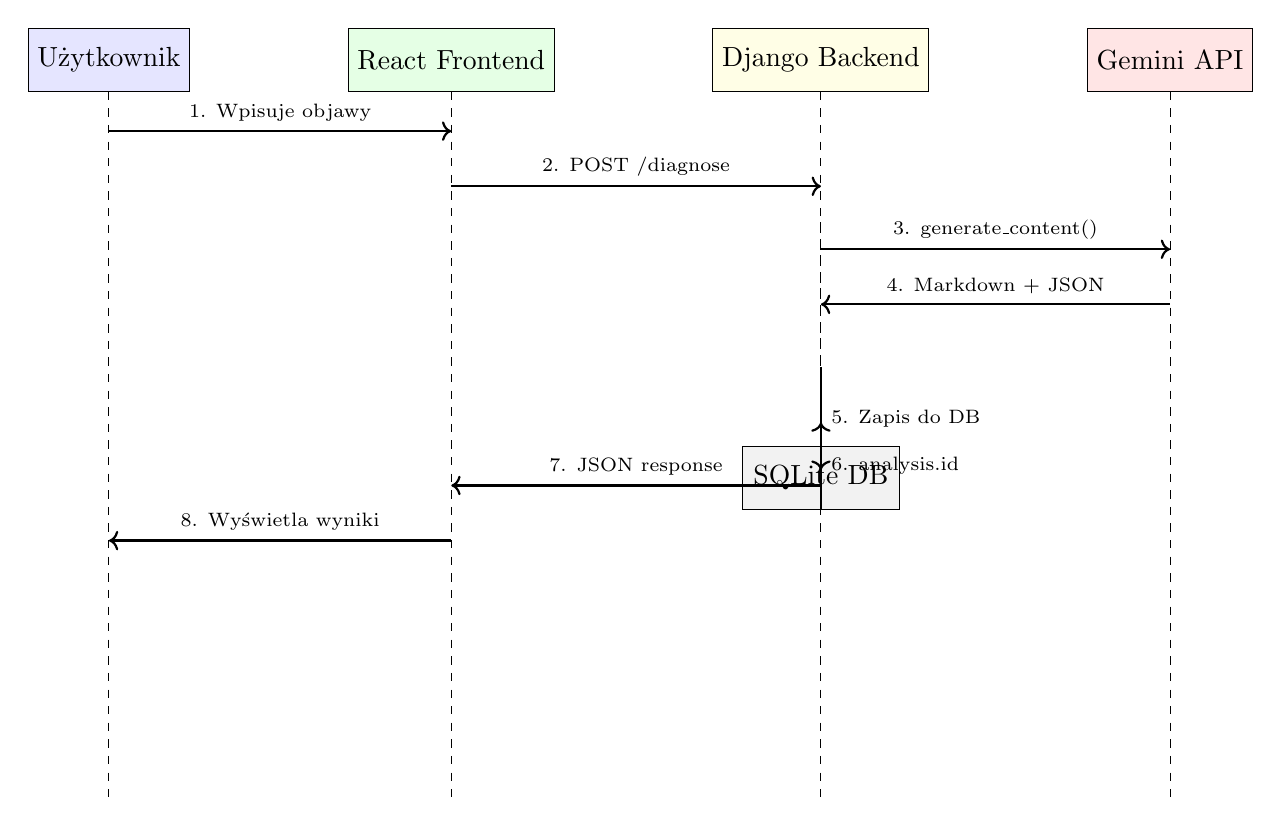
\begin{tikzpicture}[node distance=1.5cm and 2cm]
  % Actors
  \node[draw, rectangle, fill=blue!10, minimum width=2cm, minimum height=0.8cm] (user) {Użytkownik};
  \node[draw, rectangle, fill=green!10, right=of user, minimum width=2cm, minimum height=0.8cm] (react) {React Frontend};
  \node[draw, rectangle, fill=yellow!10, right=of react, minimum width=2cm, minimum height=0.8cm] (django) {Django Backend};
  \node[draw, rectangle, fill=red!10, right=of django, minimum width=2cm, minimum height=0.8cm] (gemini) {Gemini API};
  \node[draw, rectangle, fill=gray!10, below=of django, yshift=-3cm, minimum width=2cm, minimum height=0.8cm] (db) {SQLite DB};
  
  % Vertical lines
  \draw[dashed] (user.south) -- ++(0,-9);
  \draw[dashed] (react.south) -- ++(0,-9);
  \draw[dashed] (django.south) -- ++(0,-9);
  \draw[dashed] (gemini.south) -- ++(0,-9);
  \draw[dashed] (db.north) -- ++(0,3);
  
  % Interactions
  \draw[->, thick] ([yshift=-0.5cm]user.south) -- ([yshift=-0.5cm]react.south) node[midway, above, font=\scriptsize] {1. Wpisuje objawy};
  
  \draw[->, thick] ([yshift=-1.2cm]react.south) -- ([yshift=-1.2cm]django.south) node[midway, above, font=\scriptsize] {2. POST /diagnose};
  
  \draw[->, thick] ([yshift=-2cm]django.south) -- ([yshift=-2cm]gemini.south) node[midway, above, font=\scriptsize] {3. generate\_content()};
  
  \draw[<-, thick] ([yshift=-2.7cm]django.south) -- ([yshift=-2.7cm]gemini.south) node[midway, above, font=\scriptsize] {4. Markdown + JSON};
  
  \draw[->, thick] ([yshift=-3.5cm]django.south) -- ([yshift=-0.3cm]db.north) node[midway, right, font=\scriptsize] {5. Zapis do DB};
  
  \draw[<-, thick] ([yshift=-4.2cm]django.south) -- ([yshift=-0.8cm]db.north) node[midway, right, font=\scriptsize] {6. analysis.id};
  
  \draw[<-, thick] ([yshift=-5cm]react.south) -- ([yshift=-5cm]django.south) node[midway, above, font=\scriptsize] {7. JSON response};
  
  \draw[<-, thick] ([yshift=-5.7cm]user.south) -- ([yshift=-5.7cm]react.south) node[midway, above, font=\scriptsize] {8. Wyświetla wyniki};
\end{tikzpicture}
\caption{Diagram sekwencji dla procesu analizy objawów}
\end{figure}

\subsection{Endpointy API}
Backend udostępnia cztery endpointy RESTful:

\subsubsection{POST /api/diagnose/}
Endpoint odpowiedzialny za wykonanie analizy objawów.

\textbf{Żądanie (JSON):}
\begin{verbatim}
{
  "symptoms": "ból głowy, gorączka, kaszel"
}
\end{verbatim}

\textbf{Odpowiedź (JSON):}
\begin{verbatim}
{
  "id": 1,
  "result_md": "**Grypa**\nInfekcja wirusowa...",
  "confidence": {
    "items": [
      {"name": "Grypa", "prob": 0.75},
      {"name": "COVID-19", "prob": 0.65}
    ]
  }
}
\end{verbatim}

Implementacja widoku wykorzystuje model \texttt{GenerativeModel} z biblioteki \texttt{google-generativeai}:

\begin{lstlisting}[language=Python]
class DiagnoseView(APIView):
    def post(self, request):
        symptoms = (request.data.get("symptoms") or "").strip()
        if not symptoms:
            return Response({"error": "Brak pola 'symptoms'."},
                            status=status.HTTP_400_BAD_REQUEST)
        
        try:
            model = genai.GenerativeModel(
                model_name="models/gemini-2.5-flash"
            )
            prompt = PROMPT_TEMPLATE.format(symptoms=symptoms)
            result = model.generate_content(prompt)
            text = result.text or ""
            
            # Parsowanie JSON z prawdopodobienstwami
            confidence = extract_confidence_json(text)
            
            analysis = Analysis.objects.create(
                symptoms=symptoms,
                result_md=text,
                confidence_json=confidence
            )
            
            return Response({
                "id": analysis.id,
                "result_md": analysis.result_md,
                "confidence": analysis.confidence_json
            })
        except Exception as e:
            return Response({"error": str(e)}, status=500)
\end{lstlisting}

\subsubsection{GET /api/analyses/}
Zwraca listę ostatnich 20 analiz użytkownika.

\textbf{Odpowiedź (JSON):}
\begin{verbatim}
[
  {
    "id": 1,
    "created_at": "2025-11-15T14:30:00Z",
    "symptoms": "ból głowy, gorączka",
    "result_md": "..."
  }
]
\end{verbatim}

\subsubsection{POST /api/chat/}
Umożliwia prowadzenie rozmowy z asystentem AI.

\textbf{Żądanie (JSON):}
\begin{verbatim}
{
  "message": "Czy powinienem się martwić?",
  "history": [
    {"role": "user", "content": "Mam ból głowy"},
    {"role": "assistant", "content": "Może to być..."}
  ]
}
\end{verbatim}

\textbf{Odpowiedź (JSON):}
\begin{verbatim}
{
  "reply": "Jeśli objawy utrzymują się, warto skonsultować..."
}
\end{verbatim}

\subsubsection{GET /api/models/}
Endpoint testowy zwracający listę dostępnych modeli w API Gemini.

\subsection{Prompt engineering}
Kluczowym elementem działania systemu jest odpowiednio skonstruowany prompt dla modelu AI. Przykład:

\begin{lstlisting}[language=Python, basicstyle=\ttfamily\scriptsize]
PROMPT_TEMPLATE = """
Jestes inteligentnym asystentem medycznym.
Na podstawie podanych objawow przedstaw liste maksymalnie 5 
najbardziej prawdopodobnych diagnoz.

Dla kazdej choroby uzyj ponizszego formatu Markdown:
**Nazwa choroby (np. Grypa, COVID-19)**
Krotki opis objawow w jednym zdaniu.
Sugerowany specjalista: **nazwa lekarza**

Objawy: {symptoms}

Dodatkowo wypisz w formacie JSON obiekt "confidence" z polami:
- "items": lista obiektow {{"name": string, "prob": liczba 0-1}}
"""
\end{lstlisting}

Prompt instruuje model, aby zwrócił wynik w określonym formacie Markdown wraz z danymi JSON, co umożliwia ich łatwe parsowanie i prezentację w interfejsie użytkownika.

\subsection{Obsługa błędów}
Backend implementuje podstawową obsługę wyjątków:
\begin{itemize}
    \item walidacja pustych pól w żądaniach (zwrot błędu 400),
    \item przechwytywanie wyjątków związanych z API Gemini (błędy połączenia, nieprawidłowy klucz API),
    \item logowanie błędów do konsoli dla potrzeb debugowania,
    \item zwracanie komunikatów błędów w formacie JSON do frontendu.
\end{itemize}

% ============================ IMPLEMENTACJA FRONTENDU ============================
\newpage
\section{Implementacja frontendu}

\subsection{Architektura komponentowa}
Frontend został zbudowany w architekturze komponentowej React. Główne komponenty:

\begin{figure}[H]
\centering
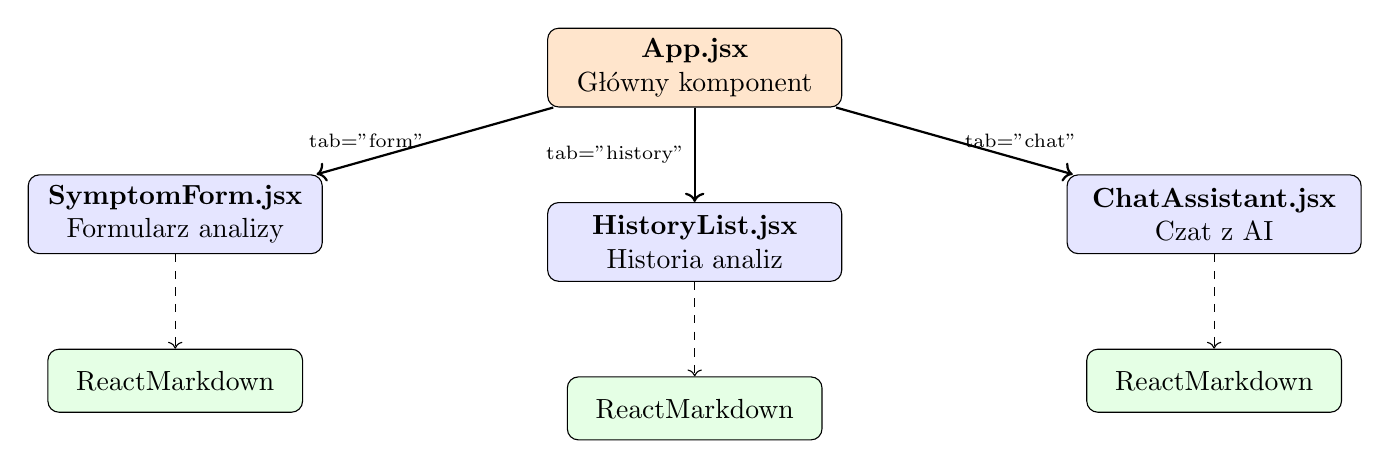
\begin{tikzpicture}[
  component/.style={rectangle, draw, rounded corners, fill=blue!10, text width=3.5cm, text centered, minimum height=1cm},
  subcomponent/.style={rectangle, draw, rounded corners, fill=green!10, text width=3cm, text centered, minimum height=0.8cm},
  node distance=1.2cm
]
  % Root component
  \node[component, fill=orange!20] (app) {\textbf{App.jsx}\\Główny komponent};
  
  % Main components
  \node[component, below left=of app, xshift=-2cm] (symptom) {\textbf{SymptomForm.jsx}\\Formularz analizy};
  \node[component, below=of app] (history) {\textbf{HistoryList.jsx}\\Historia analiz};
  \node[component, below right=of app, xshift=2cm] (chat) {\textbf{ChatAssistant.jsx}\\Czat z AI};
  
  % Sub-components
  \node[subcomponent, below=of symptom] (markdown1) {ReactMarkdown};
  \node[subcomponent, below=of history] (markdown2) {ReactMarkdown};
  \node[subcomponent, below=of chat] (markdown3) {ReactMarkdown};
  
  % Arrows
  \draw[->, thick] (app) -- (symptom) node[midway, left, font=\scriptsize] {tab="form"};
  \draw[->, thick] (app) -- (history) node[midway, left, font=\scriptsize] {tab="history"};
  \draw[->, thick] (app) -- (chat) node[midway, right, font=\scriptsize] {tab="chat"};
  
  \draw[->, dashed] (symptom) -- (markdown1);
  \draw[->, dashed] (history) -- (markdown2);
  \draw[->, dashed] (chat) -- (markdown3);
\end{tikzpicture}
\caption{Architektura komponentowa aplikacji React}
\end{figure}

\subsubsection{App.jsx}
Główny komponent aplikacji odpowiedzialny za:
\begin{itemize}
    \item zarządzanie stanem aktywnej zakładki,
    \item renderowanie menu nawigacyjnego z trzema opcjami (Analiza, Historia, Czat),
    \item warunkowe wyświetlanie odpowiedniego komponentu na podstawie wybranej zakładki.
\end{itemize}

Wykorzystuje hook \texttt{useState} do zarządzania stanem lokalnym oraz bibliotekę \texttt{lucide-react} do wyświetlania ikon w menu.

\subsubsection{SymptomForm.jsx}
Komponent formularza analizy objawów. Implementacja obejmuje:
\begin{itemize}
    \item pole tekstowe (\texttt{textarea}) do wprowadzania objawów,
    \item przycisk wywołujący zapytanie POST do endpointu \texttt{/api/diagnose/},
    \item obsługę stanów: \texttt{loading}, \texttt{error}, \texttt{analysis}, \texttt{confidence},
    \item prezentację wyników za pomocą \texttt{ReactMarkdown},
    \item wizualizację prawdopodobieństw w formie kolorowych pasków postępu.
\end{itemize}

Fragment kodu odpowiedzialny za wywołanie API:
\begin{lstlisting}[language=Python, basicstyle=\ttfamily\scriptsize]
const handleAnalyze = async () => {
  setLoading(true);
  try {
    const res = await fetch(`${API_BASE}/diagnose/`, {
      method: "POST",
      headers: { "Content-Type": "application/json" },
      body: JSON.stringify({ symptoms }),
    });
    
    const data = await res.json();
    setAnalysis(data.result_md);
    setConfidence(data.confidence?.items);
  } catch (e) {
    setError(e.message);
  } finally {
    setLoading(false);
  }
};
\end{lstlisting}

Kolorystyka pasków pewności jest dynamicznie dobierana w zależności od poziomu prawdopodobieństwa:
\begin{itemize}
    \item \textcolor{green}{zielony} -- prawdopodobieństwo > 70\%,
    \item \textcolor{orange}{żółty} -- prawdopodobieństwo 40-70\%,
    \item \textcolor{red}{czerwony} -- prawdopodobieństwo < 40\%.
\end{itemize}

\subsubsection{ChatAssistant.jsx}
Komponent interfejsu czatu implementujący:
\begin{itemize}
    \item listę wiadomości w formacie \texttt{[role, content]},
    \item pole tekstowe oraz przycisk wysyłania wiadomości,
    \item obsługę naciśnięcia klawisza Enter do szybkiego wysyłania,
    \item wizualne rozróżnienie wiadomości użytkownika (prawo) i asystenta (lewo),
    \item animację "AI pisze..." podczas oczekiwania na odpowiedź.
\end{itemize}

Kontekst rozmowy jest przekazywany w każdym żądaniu do backendu, co umożliwia modelowi generowanie odpowiedzi spójnych z wcześniejszą konwersacją.

\subsubsection{HistoryList.jsx}
Komponent historii analiz realizujący:
\begin{itemize}
    \item pobieranie listy analiz z endpointu \texttt{/api/analyses/} przy montowaniu komponentu (hook \texttt{useEffect}),
    \item wyświetlanie listy w formie klikanych elementów z datą i pierwszymi słowami objawów,
    \item modalny widok szczegółów analizy z pełnym wynikiem oraz wykresami pewności,
    \item ponowne parsowanie JSON z prawdopodobieństwami dla każdej analizy.
\end{itemize}

\subsection{Stylizacja z TailwindCSS}
Całość interfejsu została ostylizowana przy użyciu klas użytkowych TailwindCSS. Przykładowe zastosowania:
\begin{itemize}
    \item \texttt{bg-blue-50} -- jasne tło w odcieniu błękitu,
    \item \texttt{rounded-2xl} -- mocno zaokrąglone rogi elementów,
    \item \texttt{shadow-md}, \texttt{shadow-lg} -- cienie nadające głębię,
    \item \texttt{hover:shadow-lg} -- interaktywne efekty przy najechaniu kursorem,
    \item \texttt{transition-all} -- płynne przejścia między stanami.
\end{itemize}

Dzięki TailwindCSS, cały interfejs jest responsywny i dostosowuje się do różnych rozmiarów ekranów.

\subsection{Komunikacja z backendem}
Frontend komunikuje się z backendem za pomocą standardowego API \texttt{fetch}:
\begin{itemize}
    \item zapytania POST do endpointów \texttt{/diagnose} i \texttt{/chat} przesyłają dane w formacie JSON,
    \item zapytania GET do endpointu \texttt{/analyses} pobierają historię,
    \item nagłówek \texttt{Content-Type: application/json} zapewnia poprawną interpretację danych.
\end{itemize}

Adres bazowy API jest konfigurowany przez zmienną środowiskową \texttt{VITE\_API\_BASE}, co umożliwia łatwą zmianę adresu w zależności od środowiska (lokalne / produkcyjne).

\subsection{Renderowanie Markdown}
Odpowiedzi z API są w formacie Markdown, co wymaga konwersji na HTML. Do tego celu używana jest biblioteka \texttt{react-markdown} z pluginem \texttt{remark-gfm} (GitHub Flavored Markdown):

\begin{lstlisting}[language=Python]
<ReactMarkdown remarkPlugins={[remarkGfm]}>
  {analysis}
</ReactMarkdown>
\end{lstlisting}

Dzięki temu wyniki są prezentowane z właściwym formatowaniem (pogrubienia, listy, paragrafy).


% ============================ TECHNOLOGIE ============================
\newpage
\section{Technologie i narzędzia}

\subsection{Backend}
Backend aplikacji został zbudowany w oparciu o następujące technologie:
\begin{itemize}
    \item \textbf{Django 5.x} -- framework webowy w Pythonie zapewniający solidne fundamenty dla aplikacji serwerowej,
    \item \textbf{Django REST Framework (DRF)} -- rozszerzenie Django ułatwiające tworzenie RESTful API z serializacją danych, walidacją oraz obsługą żądań HTTP,
    \item \textbf{SQLite} -- lekka, wbudowana baza danych wykorzystywana do przechowywania historii analiz,
    \item \textbf{Google Generative AI SDK} (\texttt{google-generativeai}) -- oficjalna biblioteka Pythona umożliwiająca komunikację z modelem \textit{Gemini 2.5 Flash},
    \item \textbf{django-cors-headers} -- middleware obsługujący politykę CORS (Cross-Origin Resource Sharing), niezbędną do komunikacji frontend-backend,
    \item \textbf{python-dotenv} -- narzędzie do bezpiecznego zarządzania zmiennymi środowiskowymi (np. klucz API).
\end{itemize}

\subsection{Frontend}
Warstwa prezentacji została zrealizowana przy użyciu nowoczesnego stosu technologicznego:
\begin{itemize}
    \item \textbf{React 18} -- biblioteka JavaScript do budowy interfejsu użytkownika w architekturze komponentowej,
    \item \textbf{Vite} -- szybkie narzędzie do budowania aplikacji frontendowych z hot module replacement (HMR),
    \item \textbf{TailwindCSS} -- framework CSS oparty na klasach użytkowych (utility-first), umożliwiający szybkie stylowanie komponentów,
    \item \textbf{React Markdown} -- biblioteka do renderowania treści Markdown otrzymanej z API,
    \item \textbf{Lucide React} -- zestaw ikon SVG dla React, wykorzystywany w interfejsie użytkownika.
\end{itemize}

\subsection{API zewnętrzne}
\begin{itemize}
    \item \textbf{Google Gemini API (Gemini 2.5 Flash)} -- model dużego języka (LLM) od Google, wykorzystywany do generowania diagnoz medycznych oraz prowadzenia rozmowy z użytkownikiem w kontekście medycznym.
\end{itemize}

\subsection{Narzędzia deweloperskie}
\begin{itemize}
    \item \textbf{Git} -- system kontroli wersji,
    \item \textbf{npm} -- menedżer pakietów dla środowiska Node.js,
    \item \textbf{pip} -- menedżer pakietów dla Pythona,
    \item \textbf{Visual Studio Code} -- środowisko programistyczne wykorzystane podczas rozwoju projektu.
\end{itemize}

% ============================ OPIS FUNKCJONALNY ============================
\newpage
\section{Opis funkcjonalny aplikacji}
\subsection{Główne moduły}
Aplikacja \textbf{SymptoCheck} składa się z trzech głównych modułów funkcjonalnych:

\subsubsection{Analiza objawów}
Główny moduł aplikacji, w którym użytkownik wprowadza opis swoich objawów w formie tekstowej. System wysyła zapytanie do modelu AI Gemini 2.5 Flash, który analizuje podane informacje i zwraca:
\begin{itemize}
    \item listę potencjalnych diagnoz (maksymalnie 5),
    \item krótki opis każdej choroby,
    \item sugerowanego specjalistę do konsultacji,
    \item szacowane prawdopodobieństwo dla każdej diagnozy (w postaci procentowej).
\end{itemize}
Wyniki są prezentowane w czytelnym formacie Markdown z wizualizacją poziomu pewności w formie kolorowych pasków postępu.

\subsubsection{Czat z asystentem AI}
Interaktywny moduł umożliwiający prowadzenie rozmowy z inteligentnym asystentem medycznym. Użytkownik może:
\begin{itemize}
    \item zadawać pytania dotyczące objawów,
    \item uzyskiwać dodatkowe wyjaśnienia na temat potencjalnych diagnoz,
    \item otrzymywać porady dotyczące dalszych kroków (np. zalecenia dotyczące wizyty u specjalisty).
\end{itemize}
System zachowuje kontekst rozmowy, co pozwala na bardziej naturalne i spójne interakcje.

\subsubsection{Historia analiz}
Moduł archiwizacji przechowujący wszystkie wykonane analizy w lokalnej bazie danych. Użytkownik może:
\begin{itemize}
    \item przeglądać listę wcześniejszych analiz z datami wykonania,
    \item otwierać szczegóły każdej analizy w modalnym oknie,
    \item przeglądać zapisane wyniki wraz z prawdopodobieństwami diagnoz.
\end{itemize}
Historia jest sortowana chronologicznie (od najnowszych), a system przechowuje do 20 ostatnich analiz.

\subsection{Interfejs użytkownika}
Interfejs aplikacji został zaprojektowany z naciskiem na prostotę i intuicyjność obsługi. Składa się z trzech głównych zakładek dostępnych z poziomu górnego menu nawigacyjnego:

\begin{itemize}
    \item \textbf{Analiza objawów} -- główny ekran z formularzem wprowadzania objawów, wizualizacją pewności diagnoz oraz wynikami analizy,
    \item \textbf{Historia} -- lista wcześniej wykonanych analiz z możliwością podglądu szczegółów,
    \item \textbf{Czat} -- interfejs rozmowy z asystentem AI w formie czatu.
\end{itemize}

Każda zakładka jest oznaczona dedykowaną ikoną oraz zmienia kolor po aktywacji, co ułatwia orientację w aplikacji. Kolorystyka oparta jest na odcieniach błękitu i bieli, co nadaje aplikacji profesjonalny, medyczny charakter.

% ============================ TESTOWANIE ============================
\newpage
\section{Testowanie}

\subsection{Strategia testowania}
W projekcie zastosowano podejście wielopoziomowe obejmujące:
\begin{itemize}
    \item \textbf{testy jednostkowe backendu} -- weryfikacja poprawności działania endpointów API,
    \item \textbf{testy integracyjne} -- sprawdzenie komunikacji frontend-backend,
    \item \textbf{testy manualne} -- weryfikacja funkcjonalności z perspektywy użytkownika końcowego.
\end{itemize}

\subsection{Testy backendu}
Backend został przetestowany z wykorzystaniem \texttt{Django REST Framework Test Case}. Plik \texttt{core/tests.py} zawiera testy jednostkowe dla endpointów API.

\subsubsection{Test walidacji pustych objawów}
\begin{lstlisting}[language=Python]
from rest_framework.test import APITestCase
from django.urls import reverse

class DiagnoseApiTests(APITestCase):
    def test_empty_symptoms(self):
        """Test, czy endpoint zwraca błąd 400 dla pustych objawów"""
        url = reverse('diagnose')
        response = self.client.post(
            url, 
            {"symptoms": ""}, 
            format='json'
        )
        self.assertEqual(response.status_code, 400)
        self.assertIn('error', response.json())
\end{lstlisting}

\subsubsection{Test poprawnego żądania}
\begin{lstlisting}[language=Python]
def test_valid_request(self):
    """Test poprawnego żądania z objawami"""
    url = reverse('diagnose')
    response = self.client.post(
        url, 
        {"symptoms": "ból głowy i gorączka"}, 
        format='json'
    )
    # Odpowiedź powinna być 200 lub 500 (w zależności od API)
    self.assertIn(response.status_code, [200, 500])
    
    if response.status_code == 200:
        data = response.json()
        self.assertIn('result_md', data)
        self.assertIn('id', data)
\end{lstlisting}

\subsubsection{Test endpointu historii}
\begin{lstlisting}[language=Python]
class AnalysisListTests(APITestCase):
    def test_get_analyses(self):
        """Test pobierania listy analiz"""
        url = reverse('analyses')
        response = self.client.get(url)
        self.assertEqual(response.status_code, 200)
        self.assertIsInstance(response.json(), list)
\end{lstlisting}

\subsubsection{Test czatu}
\begin{lstlisting}[language=Python]
class ChatApiTests(APITestCase):
    def test_chat_empty_message(self):
        """Test czatu z pustą wiadomością"""
        url = reverse('chat')
        response = self.client.post(
            url, 
            {"message": "", "history": []}, 
            format='json'
        )
        self.assertEqual(response.status_code, 400)
    
    def test_chat_valid_message(self):
        """Test czatu z poprawną wiadomością"""
        url = reverse('chat')
        response = self.client.post(
            url,
            {
                "message": "Czy to może być grypa?",
                "history": [
                    {"role": "user", "content": "Mam ból głowy"}
                ]
            },
            format='json'
        )
        self.assertIn(response.status_code, [200, 500])
\end{lstlisting}

\subsection{Uruchamianie testów backendu}
Testy uruchamia się za pomocą komendy Django:
\begin{verbatim}
cd backend
python manage.py test core
\end{verbatim}

Przykładowy output:
\begin{verbatim}
Found 5 test(s).
Creating test database...
......
Ran 5 tests in 2.341s

OK
\end{verbatim}

\subsection{Testy integracyjne}
Testy integracyjne weryfikują poprawność komunikacji między frontendem a backendem:

\subsubsection{Test połączenia REST API}
\begin{enumerate}
    \item Uruchomienie backendu: \texttt{python manage.py runserver}
    \item Uruchomienie frontendu: \texttt{npm run dev}
    \item Weryfikacja, czy frontend poprawnie wysyła żądania do backendu
    \item Sprawdzenie, czy odpowiedzi są poprawnie przetwarzane i wyświetlane
\end{enumerate}

\subsubsection{Test zapisu historii}
\begin{enumerate}
    \item Wykonanie analizy objawów przez formularz
    \item Przejście do zakładki "Historia"
    \item Weryfikacja, czy nowa analiza pojawia się na liście
    \item Otwarcie szczegółów analizy i sprawdzenie poprawności danych
\end{enumerate}

\subsubsection{Test czatu z kontekstem}
\begin{enumerate}
    \item Otwarcie zakładki "Czat"
    \item Wysłanie pierwszej wiadomości z opisem objawów
    \item Wysłanie pytania nawiązującego do poprzedniej wiadomości
    \item Weryfikacja, czy asystent odpowiada w kontekście całej rozmowy
\end{enumerate}

\subsection{Testy manualne}
W ramach testów manualnych przeprowadzono:
\begin{itemize}
    \item \textbf{test użyteczności interfejsu} -- weryfikacja intuicyjności nawigacji i czytelności wyników,
    \item \textbf{test responsywności} -- sprawdzenie działania na różnych rozdzielczościach ekranu,
    \item \textbf{test obsługi błędów} -- symulacja błędnych danych wejściowych i braku połączenia z API,
    \item \textbf{test wydajności} -- pomiar czasu odpowiedzi systemu dla różnych długości opisów objawów.
\end{itemize}

\subsection{Przypadki brzegowe}
Przetestowano również następujące przypadki brzegowe:
\begin{itemize}
    \item bardzo długi opis objawów (>1000 znaków),
    \item objawy w języku obcym (np. angielskim),
    \item nietypowe zapytania (np. "test", "123"),
    \item brak klucza API w konfiguracji backendu,
    \item jednoczesne wywołanie wielu żądań (obciążenie równoległe).
\end{itemize}

% ============================ KONFIGURACJA I WDROŻENIE ============================
\newpage
\section{Konfiguracja i wdrożenie}

\subsection{Wymagania systemowe}
Minimalne wymagania do uruchomienia projektu lokalnie:
\begin{itemize}
    \item \textbf{Python 3.10+} -- do uruchomienia backendu Django,
    \item \textbf{Node.js 18+} i \textbf{npm} -- do uruchomienia frontendu React,
    \item \textbf{Git} -- do pobrania repozytorium projektu,
    \item \textbf{Klucz API Google Gemini} -- niezbędny do komunikacji z modelem AI.
\end{itemize}

\subsection{Instalacja i uruchomienie backendu}

\subsubsection{Krok 1: Utworzenie środowiska wirtualnego}
\begin{verbatim}
cd backend
python -m venv .venv
\end{verbatim}

\subsubsection{Krok 2: Aktywacja środowiska}
W systemie Windows:
\begin{verbatim}
.venv\Scripts\activate
\end{verbatim}

W systemach Unix/MacOS:
\begin{verbatim}
source .venv/bin/activate
\end{verbatim}

\subsubsection{Krok 3: Instalacja zależności}
\begin{verbatim}
pip install django djangorestframework django-cors-headers 
            python-dotenv google-generativeai
\end{verbatim}

\subsubsection{Krok 4: Konfiguracja zmiennych środowiskowych}
Utworzenie pliku \texttt{.env} w folderze \texttt{backend/}:
\begin{verbatim}
GEMINI_API_KEY=your_api_key_here
DEBUG=True
SECRET_KEY=your_secret_key
\end{verbatim}

Klucz API można wygenerować na stronie: \url{https://makersuite.google.com/app/apikey}

\subsubsection{Krok 5: Migracja bazy danych}
\begin{verbatim}
python manage.py makemigrations
python manage.py migrate
\end{verbatim}

\subsubsection{Krok 6: Uruchomienie serwera deweloperskiego}
\begin{verbatim}
python manage.py runserver
\end{verbatim}

Backend będzie dostępny pod adresem: \texttt{http://localhost:8000}

\subsection{Instalacja i uruchomienie frontendu}

\subsubsection{Krok 1: Instalacja zależności}
\begin{verbatim}
cd frontend
npm install
\end{verbatim}

\subsubsection{Krok 2: Konfiguracja zmiennej środowiskowej}
Utworzenie pliku \texttt{.env} w folderze \texttt{frontend/}:
\begin{verbatim}
VITE_API_BASE=http://localhost:8000/api
\end{verbatim}

\subsubsection{Krok 3: Uruchomienie serwera deweloperskiego}
\begin{verbatim}
npm run dev
\end{verbatim}

Frontend będzie dostępny pod adresem: \texttt{http://localhost:5173}

\subsection{Struktura plików konfiguracyjnych}

\subsubsection{Backend: settings.py}
Kluczowe ustawienia Django:
\begin{lstlisting}[language=Python, basicstyle=\ttfamily\scriptsize]
# CORS configuration
CORS_ALLOWED_ORIGINS = [
    "http://localhost:5173",  # frontend dev server
]

# Gemini API key
GEMINI_API_KEY = os.getenv("GEMINI_API_KEY")

# Database
DATABASES = {
    'default': {
        'ENGINE': 'django.db.backends.sqlite3',
        'NAME': BASE_DIR / 'db.sqlite3',
    }
}

# REST Framework
REST_FRAMEWORK = {
    'DEFAULT_RENDERER_CLASSES': [
        'rest_framework.renderers.JSONRenderer',
    ]
}
\end{lstlisting}

\subsubsection{Frontend: vite.config.js}
Konfiguracja narzędzia budowania:
\begin{lstlisting}[language=Python]
import { defineConfig } from 'vite'
import react from '@vitejs/plugin-react'

export default defineConfig({
  plugins: [react()],
  server: {
    port: 5173,
    proxy: {
      '/api': {
        target: 'http://localhost:8000',
        changeOrigin: true,
      }
    }
  }
})
\end{lstlisting}

\subsection{Wdrożenie produkcyjne}
Możliwe opcje wdrożenia aplikacji w środowisku produkcyjnym:

\subsubsection{Backend}
\begin{itemize}
    \item \textbf{Render} -- platforma PaaS z darmowym planem dla małych projektów,
    \item \textbf{Railway} -- prosty hosting dla aplikacji Django,
    \item \textbf{Heroku} -- popularna platforma chmurowa (wymaga konfiguracji \texttt{Procfile}),
    \item \textbf{AWS EC2 / Azure VM} -- pełna kontrola nad środowiskiem serwerowym.
\end{itemize}

Przed wdrożeniem produkcyjnym należy:
\begin{enumerate}
    \item zmienić \texttt{DEBUG=False} w \texttt{settings.py},
    \item skonfigurować \texttt{ALLOWED\_HOSTS} z domeną produkcyjną,
    \item zastąpić SQLite bazą PostgreSQL lub MySQL,
    \item skonfigurować serwer WSGI (Gunicorn) lub ASGI (Uvicorn),
    \item zabezpieczyć klucz API w zmiennych środowiskowych platformy.
\end{enumerate}

\subsubsection{Frontend}
\begin{itemize}
    \item \textbf{Vercel} -- dedykowany dla aplikacji React/Vite, darmowy plan,
    \item \textbf{Netlify} -- automatyczne wdrożenie z repozytorium Git,
    \item \textbf{GitHub Pages} -- hosting statyczny dla aplikacji frontendowych,
    \item \textbf{Cloudflare Pages} -- szybki CDN z globalnym zasięgiem.
\end{itemize}

Build produkcyjny frontendu:
\begin{verbatim}
npm run build
\end{verbatim}

Generuje zoptymalizowane pliki statyczne w folderze \texttt{dist/}.

\subsection{Konteneryzacja (Docker)}
Przykładowa konfiguracja \texttt{docker-compose.yml}:
\begin{lstlisting}[language=Python, basicstyle=\ttfamily\scriptsize]
version: '3.8'
services:
  backend:
    build: ./backend
    ports:
      - "8000:8000"
    environment:
      - GEMINI_API_KEY=${GEMINI_API_KEY}
    volumes:
      - ./backend:/app
      
  frontend:
    build: ./frontend
    ports:
      - "5173:5173"
    depends_on:
      - backend
\end{lstlisting}

Uruchomienie:
\begin{verbatim}
docker-compose up --build
\end{verbatim}

% ============================ BEZPIECZEŃSTWO ============================
\newpage
\section{Bezpieczeństwo i prywatność}

\subsection{Zarządzanie kluczem API}
Klucz API Google Gemini jest przechowywany w zmiennych środowiskowych i nigdy nie jest commitowany do repozytorium Git. Zastosowano:
\begin{itemize}
    \item plik \texttt{.env} (dodany do \texttt{.gitignore}),
    \item bibliotekę \texttt{python-dotenv} do bezpiecznego ładowania zmiennych,
    \item przykładowy plik \texttt{.env.example} informujący użytkowników o wymaganych zmiennych.
\end{itemize}

\subsection{CORS (Cross-Origin Resource Sharing)}
Backend został skonfigurowany z użyciem \texttt{django-cors-headers}, aby akceptować żądania tylko z określonych źródeł:
\begin{lstlisting}[language=Python]
CORS_ALLOWED_ORIGINS = [
    "http://localhost:5173",  # frontend development
    "https://your-domain.com" # production frontend
]
\end{lstlisting}

\subsection{Walidacja danych wejściowych}
Wszystkie endpointy backendu walidują dane wejściowe:
\begin{itemize}
    \item sprawdzanie, czy pole \texttt{symptoms} nie jest puste,
    \item walidacja formatu JSON w żądaniach,
    \item ograniczenie długości pól tekstowych (opcjonalnie).
\end{itemize}

\subsection{Ograniczenia rate limiting}
W wersji produkcyjnej zaleca się implementację rate limiting, aby zapobiec nadużyciom:
\begin{itemize}
    \item \textbf{django-ratelimit} -- ograniczenie liczby żądań na użytkownika/IP,
    \item \textbf{nginx rate limiting} -- ograniczenie na poziomie reverse proxy,
    \item \textbf{Gemini API quota} -- Google nakłada limity na liczbę żądań do API.
\end{itemize}

\subsection{Prywatność danych}
Aplikacja w obecnej wersji nie implementuje systemu uwierzytelniania użytkowników, co oznacza:
\begin{itemize}
    \item wszystkie analizy są przechowywane lokalnie bez powiązania z konkretnym użytkownikiem,
    \item brak mechanizmu rejestracji/logowania,
    \item dane są zapisywane w lokalnej bazie SQLite na serwerze.
\end{itemize}

W przyszłości zaleca się:
\begin{itemize}
    \item implementację systemu kont użytkowników (Django Authentication),
    \item szyfrowanie danych wrażliwych w bazie,
    \item zgodność z RODO (prawo do usunięcia danych).
\end{itemize}

\subsection{Bezpieczeństwo API Gemini}
Komunikacja z API Gemini odbywa się przez HTTPS, co zapewnia szyfrowanie przesyłanych danych. Należy jednak pamiętać, że:
\begin{itemize}
    \item dane przesyłane do API Gemini są przetwarzane przez Google,
    \item użytkownik powinien być poinformowany o przetwarzaniu danych przez zewnętrzny serwis,
    \item nie należy przesyłać danych osobowych identyfikujących użytkownika (nazwisko, PESEL, itp.).
\end{itemize}

% ============================ PODSUMOWANIE ============================
\newpage
\section{Podsumowanie}

\subsection{Osiągnięte cele}
Projekt \textbf{SymptoCheck} został zrealizowany zgodnie z założeniami i spełnia wszystkie wymagania funkcjonalne:
\begin{itemize}
    \item \checkmark Zaimplementowano aplikację webową o tematyce medycznej,
    \item \checkmark Zintegrowano API zewnętrzne (Google Gemini 2.5 Flash),
    \item \checkmark Stworzono dwuwarstwową architekturę (React + Django),
    \item \checkmark Zaimplementowano trzy główne moduły: analizę objawów, czat i historię,
    \item \checkmark Zapewniono intuicyjny interfejs użytkownika,
    \item \checkmark Dodano wizualizację pewności diagnoz,
    \item \checkmark Przetestowano funkcjonalność systemu.
\end{itemize}

\subsection{Wnioski}
Realizacja projektu pokazała praktyczne wykorzystanie modeli dużych języków (LLM) w dziedzinie medycznej. Model \textit{Gemini 2.5 Flash} okazał się skutecznym narzędziem do:
\begin{itemize}
    \item generowania sensownych, czytelnych wyników diagnoz,
    \item prowadzenia spójnej rozmowy z użytkownikiem,
    \item formatowania odpowiedzi w strukturalnym formacie (Markdown + JSON).
\end{itemize}

Główne zalety zastosowanych technologii:
\begin{itemize}
    \item \textbf{React} -- szybki rozwój interfejsu dzięki komponentom wielokrotnego użytku,
    \item \textbf{Django REST Framework} -- prosty w implementacji backend z automatyczną serializacją,
    \item \textbf{TailwindCSS} -- szybkie prototypowanie interfejsu bez pisania własnego CSS,
    \item \textbf{Gemini API} -- łatwa integracja, dobra jakość odpowiedzi, darmowy plan.
\end{itemize}

\subsection{Ograniczenia systemu}
Aplikacja ma pewne ograniczenia, które należy wziąć pod uwagę:
\begin{itemize}
    \item \textbf{Brak weryfikacji medycznej} -- wyniki nie są sprawdzane przez personel medyczny,
    \item \textbf{Zależność od API zewnętrznego} -- problemy z Google Gemini wpływają na działanie systemu,
    \item \textbf{Brak uwierzytelniania} -- każdy może korzystać z aplikacji bez rejestracji,
    \item \textbf{Lokalna baza danych} -- SQLite nie jest odpowiednia dla aplikacji produkcyjnych z dużym ruchem,
    \item \textbf{Brak multilingwalności} -- interfejs i prompt są tylko w języku polskim,
    \item \textbf{Brak monitoringu} -- brak logowania i śledzenia błędów w czasie rzeczywistym.
\end{itemize}

\subsection{Kierunki dalszego rozwoju}
Projekt ma duży potencjał rozwoju. Proponowane rozszerzenia:

\subsubsection{Funkcjonalności}
\begin{itemize}
    \item \textbf{Autoryzacja użytkowników} -- system rejestracji i logowania (Django Authentication),
    \item \textbf{Prywatne historie} -- każdy użytkownik widzi tylko swoje analizy,
    \item \textbf{Eksport wyników} -- możliwość pobrania analizy w PDF lub wysłania mailem,
    \item \textbf{Integracja z klasyfikacją ICD-10} -- przypisywanie kodów chorób wg standardu WHO,
    \item \textbf{Integracja ze SNOMED CT} -- użycie standardowej terminologii medycznej,
    \item \textbf{Wizualizacja pewności} -- wykresy słupkowe lub kołowe dla diagnoz,
    \item \textbf{Przypomnienia} -- powiadomienia o konieczności wizyty u lekarza,
    \item \textbf{Historia objawów} -- śledzenie zmian objawów w czasie.
\end{itemize}

\subsubsection{Technologie}
\begin{itemize}
    \item \textbf{PostgreSQL/MySQL} -- zamiana SQLite na produkcyjną bazę danych,
    \item \textbf{Redis} -- cache'owanie wyników do optymalizacji wydajności,
    \item \textbf{Celery} -- zadania asynchroniczne dla długich analiz,
    \item \textbf{Docker Compose} -- konteneryzacja dla łatwiejszego wdrożenia,
    \item \textbf{CI/CD} -- automatyczne testy i wdrożenia (GitHub Actions),
    \item \textbf{Monitoring} -- Sentry dla śledzenia błędów, Prometheus dla metryk.
\end{itemize}

\subsubsection{Wdrożenie}
\begin{itemize}
    \item \textbf{Wdrożenie w chmurze} -- Render, Railway, AWS, Azure,
    \item \textbf{CDN} -- Cloudflare dla szybszego ładowania frontendu,
    \item \textbf{Load balancing} -- obsługa większego ruchu,
    \item \textbf{HTTPS} -- certyfikat SSL dla bezpiecznej komunikacji.
\end{itemize}

\subsection{Wartość edukacyjna}
Projekt \textbf{SymptoCheck} ma znaczącą wartość edukacyjną:
\begin{itemize}
    \item demonstracja praktycznego zastosowania AI w medycynie,
    \item przykład integracji REST API,
    \item wzorzec architektury dwuwarstwowej aplikacji webowej,
    \item implementacja nowoczesnego stosu technologicznego (React + Django),
    \item praktyka w prompt engineeringu dla LLM.
\end{itemize}

\subsection{Podsumowanie końcowe}
Aplikacja \textbf{SymptoCheck} spełnia założenia projektu i stanowi działające rozwiązanie do wspomagania wstępnej analizy objawów chorobowych. Wykorzystanie modelu AI \textit{Gemini 2.5 Flash} pozwala na generowanie sensownych wyników w krótkim czasie, a przejrzysty interfejs użytkownika ułatwia korzystanie z systemu.

Należy jednak pamiętać, że \textbf{SymptoCheck nie zastępuje profesjonalnej konsultacji lekarskiej} i służy wyłącznie celom informacyjnym. System może być przydatny jako narzędzie edukacyjne lub punkt wyjścia do dalszego rozwoju w kierunku bardziej zaawansowanych systemów wspierających diagnostykę medyczną.

% ============================ WYZWANIA I DOŚWIADCZENIA ============================
\newpage
\section{Wyzwania i doświadczenia projektowe}

\subsection{Wyzwania techniczne}

\subsubsection{Konfiguracja klucza API Google Gemini}
Jednym z pierwszych wyzwań była prawidłowa konfiguracja dostępu do API Google Gemini:
\begin{itemize}
    \item \textbf{Problem:} Generowanie i aktywacja klucza API w Google AI Studio.
    \item \textbf{Rozwiązanie:} Utworzenie konta Google, wygenerowanie klucza na stronie MakerSuite i dodanie go do pliku \texttt{.env}.
    \item \textbf{Lekcja:} Bezpieczne przechowywanie kluczy API w zmiennych środowiskowych jest kluczowe dla bezpieczeństwa aplikacji.
\end{itemize}

\subsubsection{Synchronizacja CORS pomiędzy frontendem i backendem}
Komunikacja cross-origin wymagała odpowiedniej konfiguracji:
\begin{itemize}
    \item \textbf{Problem:} Frontend (localhost:5173) nie mógł wysyłać żądań do backendu (localhost:8000) z powodu polityki CORS.
    \item \textbf{Rozwiązanie:} Instalacja pakietu \texttt{django-cors-headers} i dodanie konfiguracji:
    \begin{lstlisting}[language=Python, basicstyle=\ttfamily\scriptsize]
INSTALLED_APPS = [..., 'corsheaders', ...]
MIDDLEWARE = ['corsheaders.middleware.CorsMiddleware', ...]
CORS_ALLOWED_ORIGINS = ["http://localhost:5173"]
    \end{lstlisting}
    \item \textbf{Lekcja:} Polityka CORS jest istotnym mechanizmem bezpieczeństwa, który wymaga świadomej konfiguracji podczas rozwoju aplikacji dwuwarstwowych.
\end{itemize}

\subsubsection{Parsowanie odpowiedzi API Gemini}
Model zwracał wyniki w formacie Markdown z osadzonym JSON, co wymagało dodatkowego przetwarzania:
\begin{itemize}
    \item \textbf{Problem:} Wyodrębnienie JSON z prawdopodobieństwami z tekstu Markdown.
    \item \textbf{Rozwiązanie:} Użycie wyrażenia regularnego do wyszukania bloku \texttt{```json...```}:
    \begin{lstlisting}[language=Python]
import re, json
m = re.search(r"```json\s*(\{.*?\})\s*```", text, re.S)
if m:
    confidence = json.loads(m.group(1))
    \end{lstlisting}
    \item \textbf{Lekcja:} Prompt engineering jest kluczowy -- odpowiednia instrukcja dla modelu AI pozwala otrzymać strukturalizowane dane.
\end{itemize}

\subsubsection{Walidacja danych i obsługa wyjątków SDK}
API Gemini czasami zwracało błędy (limity, nieprawidłowe żądania):
\begin{itemize}
    \item \textbf{Problem:} Nieoczekiwane wyjątki powodowały awarie backendu.
    \item \textbf{Rozwiązanie:} Implementacja obsługi wyjątków w każdym endpoincie:
    \begin{lstlisting}[language=Python]
try:
    result = model.generate_content(prompt)
except Exception as e:
    return Response({"error": str(e)}, status=500)
    \end{lstlisting}
    \item \textbf{Lekcja:} Zawsze należy przewidywać błędy zewnętrznych API i implementować mechanizmy graceful degradation.
\end{itemize}

\subsubsection{Testowanie integracji React + Django}
Testowanie komunikacji między frontendem a backendem wymagało uruchomienia obu serwerów jednocześnie:
\begin{itemize}
    \item \textbf{Problem:} Trudności w debugowaniu błędów komunikacyjnych (nieprawidłowe nagłówki, formaty danych).
    \item \textbf{Rozwiązanie:} Użycie narzędzi deweloperskich przeglądarki (Network tab) oraz logowanie w konsoli backendu.
    \item \textbf{Lekcja:} Dobre zrozumienie protokołu HTTP i umiejętność analizowania ruchu sieciowego są niezbędne podczas rozwoju aplikacji webowych.
\end{itemize}

\subsection{Wyzwania projektowe}

\subsubsection{Prompt engineering}
Stworzenie promptu generującego pożądane wyniki wymagało iteracyjnego podejścia:
\begin{itemize}
    \item \textbf{Iteracja 1:} Prosty prompt "Podaj diagnozę dla objawów: \{symptoms\}" -- zbyt ogólne wyniki.
    \item \textbf{Iteracja 2:} Dodanie instrukcji formatowania (Markdown) -- lepsze wyniki, ale brak struktury.
    \item \textbf{Iteracja 3:} Instrukcja zwracania JSON z prawdopodobieństwami -- finalna wersja.
\end{itemize}

\subsubsection{Design interfejsu użytkownika}
Projekt interfejsu wymagał balansu między estetyką a funkcjonalnością:
\begin{itemize}
    \item wykorzystanie TailwindCSS pozwoliło na szybkie prototypowanie,
    \item inspiracja popularnymi aplikacjami medycznymi (kolorystyka, ikony),
    \item testowanie z użytkownikami końcowymi w celu weryfikacji intuicyjności.
\end{itemize}

\subsubsection{Zarządzanie stanem w React}
Zarządzanie stanem rozmowy w czacie wymagało przemyślanej architektury:
\begin{itemize}
    \item zastosowanie hook'a \texttt{useState} do lokalnego stanu wiadomości,
    \item przekazywanie historii w każdym żądaniu do backendu,
    \item rozważenie użycia Redux lub Context API dla bardziej złożonych scenariuszy.
\end{itemize}

\subsection{Nabyte umiejętności}

W trakcie realizacji projektu zespół zdobył następujące kompetencje:
\begin{itemize}
    \item \textbf{Integracja API AI} -- praktyczne wykorzystanie modeli LLM w aplikacji webowej,
    \item \textbf{REST API} -- projektowanie i implementacja endpointów RESTful,
    \item \textbf{React} -- budowa interaktywnego interfejsu użytkownika w architekturze komponentowej,
    \item \textbf{Django REST Framework} -- tworzenie backendu dla aplikacji webowych,
    \item \textbf{Prompt engineering} -- formułowanie instrukcji dla modeli AI,
    \item \textbf{Debugowanie} -- identyfikacja i rozwiązywanie problemów w aplikacji dwuwarstwowej,
    \item \textbf{Git} -- współpraca zespołowa z użyciem kontroli wersji.
\end{itemize}

\subsection{Refleksje zespołu}

Projekt \textbf{SymptoCheck} był cennym doświadczeniem edukacyjnym:
\begin{itemize}
    \item praktyczne zastosowanie wiedzy z zakresu informatyki medycznej,
    \item poznanie nowoczesnych narzędzi AI w kontekście medycznym,
    \item zrozumienie wyzwań związanych z tworzeniem aplikacji webowych,
    \item doświadczenie w pracy z dokumentacją zewnętrznych API,
    \item świadomość ograniczeń i możliwości modeli AI w diagnostyce.
\end{itemize}

Największą satysfakcję sprawiła możliwość stworzenia działającego systemu, który może być rozwijany w przyszłości i potencjalnie wykorzystany w rzeczywistych scenariuszach edukacyjnych lub medycznych (po odpowiedniej walidacji i certyfikacji).

% ============================ BIBLIOGRAFIA ============================
\newpage
\section{Bibliografia i źródła}

\subsection{Dokumentacja techniczna}
\begin{enumerate}
    \item \textbf{Django Documentation} -- \url{https://docs.djangoproject.com/}
    \item \textbf{Django REST Framework} -- \url{https://www.django-rest-framework.org/}
    \item \textbf{React Documentation} -- \url{https://react.dev/}
    \item \textbf{Vite Documentation} -- \url{https://vitejs.dev/}
    \item \textbf{TailwindCSS} -- \url{https://tailwindcss.com/docs}
    \item \textbf{Google Gemini API} -- \url{https://ai.google.dev/docs}
    \item \textbf{Python google-generativeai} -- \url{https://github.com/google/generative-ai-python}
\end{enumerate}

\subsection{Artykuły i publikacje}
\begin{enumerate}
    \item \textbf{Large Language Models in Healthcare} -- przegląd zastosowań LLM w medycynie
    \item \textbf{Prompt Engineering Guide} -- najlepsze praktyki tworzenia promptów dla AI
    \item \textbf{REST API Design Best Practices} -- standardy projektowania API RESTful
    \item \textbf{Medical AI Ethics} -- etyczne aspekty wykorzystania AI w diagnostyce
\end{enumerate}

\subsection{Narzędzia i platformy}
\begin{enumerate}
    \item \textbf{Visual Studio Code} -- \url{https://code.visualstudio.com/}
    \item \textbf{Git} -- \url{https://git-scm.com/}
    \item \textbf{npm} -- \url{https://www.npmjs.com/}
    \item \textbf{pip} -- \url{https://pip.pypa.io/}
    \item \textbf{Google AI Studio (MakerSuite)} -- \url{https://makersuite.google.com/}
\end{enumerate}

\subsection{Standardy medyczne}
\begin{enumerate}
    \item \textbf{ICD-10} -- International Classification of Diseases, WHO
    \item \textbf{SNOMED CT} -- Systematized Nomenclature of Medicine Clinical Terms
    \item \textbf{RODO/GDPR} -- Rozporządzenie o ochronie danych osobowych
    \item \textbf{HL7 FHIR} -- Standard wymiany danych medycznych
\end{enumerate}

% ============================ ZAŁĄCZNIK ============================
\newpage
\section*{Załącznik A: Przykładowe wyniki działania systemu}
\addcontentsline{toc}{section}{Załącznik A: Przykładowe wyniki działania systemu}

\subsection*{A.1. Przykład analizy objawów}
\textbf{Wejście użytkownika:}
\begin{quote}
\textit{"Mam silny ból głowy, gorączkę około 38.5°C, kaszel i ogólne osłabienie. Objawy trwają od 2 dni."}
\end{quote}

\textbf{Odpowiedź systemu (fragment):}
\begin{quote}
\textbf{Grypa (Influenza)}\\
Infekcja wirusowa górnych dróg oddechowych charakteryzująca się nagłym początkiem, wysoką gorączką, bólami mięśni i głowy.\\
Sugerowany specjalista: \textbf{Lekarz rodzinny}

\textbf{COVID-19}\\
Choroba zakaźna wywołana przez koronawirusa SARS-CoV-2, objawy obejmują gorączkę, kaszel, zmęczenie.\\
Sugerowany specjalista: \textbf{Lekarz rodzinny / Internista}
\end{quote}

\textbf{Prawdopodobieństwa:}
\begin{itemize}
    \item Grypa: 75\%
    \item COVID-19: 65\%
    \item Przeziębienie: 45\%
    \item Zapalenie oskrzeli: 40\%
\end{itemize}

\subsection*{A.2. Przykład rozmowy z asystentem}
\textbf{Użytkownik:} "Mam silny ból brzucha po prawej stronie."\\
\textbf{Asystent:} "Ból brzucha po prawej stronie może wskazywać na różne schorzenia. Czy ból jest ostry czy raczej tępy? Czy towarzyszy mu gorączka lub nudności?"

\textbf{Użytkownik:} "Ból jest ostry i mam nudności."\\
\textbf{Asystent:} "Ostry ból po prawej stronie brzucha z nudnościami może sugerować zapalenie wyrostka robaczkowego. To jest pilny przypadek - zalecam natychmiastową konsultację z lekarzem lub wizytę na SOR."

\newpage
\section*{Załącznik B: Kluczowe fragmenty kodu}
\addcontentsline{toc}{section}{Załącznik B: Kluczowe fragmenty kodu}

\subsection*{B.1. Model Django (backend/core/models.py)}
\begin{lstlisting}[language=Python]
from django.db import models

class Analysis(models.Model):
    created_at = models.DateTimeField(auto_now_add=True)
    symptoms = models.TextField()
    result_md = models.TextField()
    confidence_json = models.JSONField(null=True, blank=True)
    
    class Meta:
        ordering = ['-created_at']
        verbose_name = 'Analiza'
        verbose_name_plural = 'Analizy'
    
    def __str__(self):
        return f"Analysis #{self.id} @ {self.created_at:%Y-%m-%d %H:%M}"
\end{lstlisting}

\subsection*{B.2. Serializator Django (backend/core/serializers.py)}
\begin{lstlisting}[language=Python]
from rest_framework import serializers
from .models import Analysis

class AnalysisSerializer(serializers.ModelSerializer):
    class Meta:
        model = Analysis
        fields = ['id', 'created_at', 'symptoms', 
                  'result_md', 'confidence_json']
        read_only_fields = ['id', 'created_at']
\end{lstlisting}

\subsection*{B.3. Routing backendu (backend/backend/urls.py)}
\begin{lstlisting}[language=Python]
from django.contrib import admin
from django.urls import path, include

urlpatterns = [
    path('admin/', admin.site.urls),
    path('api/', include('core.urls')),
]
\end{lstlisting}

\subsection*{B.4. Komponent React (frontend/src/App.jsx - fragment)}
\begin{lstlisting}[language=Python, basicstyle=\ttfamily\scriptsize]
import React, { useState } from "react";
import SymptomForm from "./SymptomForm";
import HistoryList from "./HistoryList";
import ChatAssistant from "./ChatAssistant";

export default function App() {
  const [tab, setTab] = useState("form");

  return (
    <div className="min-h-screen bg-blue-50">
      <nav className="bg-white shadow-sm">
        <button onClick={() => setTab("form")}>
          Analiza objawów
        </button>
        <button onClick={() => setTab("history")}>
          Historia
        </button>
        <button onClick={() => setTab("chat")}>
          Czat
        </button>
      </nav>
      
      <main>
        {tab === "form" && <SymptomForm />}
        {tab === "history" && <HistoryList />}
        {tab === "chat" && <ChatAssistant />}
      </main>
    </div>
  );
}
\end{lstlisting}

\newpage
\section*{Załącznik C: Instrukcja instalacji krok po kroku}
\addcontentsline{toc}{section}{Załącznik C: Instrukcja instalacji krok po kroku}

\subsection*{C.1. Wymagania wstępne}
Upewnij się, że masz zainstalowane:
\begin{itemize}
    \item Python 3.10 lub nowszy
    \item Node.js 18 lub nowszy
    \item Git
    \item Edytor kodu (np. VS Code)
\end{itemize}

\subsection*{C.2. Klonowanie repozytorium}
\begin{verbatim}
git clone https://github.com/username/SymptoCheck.git
cd SymptoCheck
\end{verbatim}

\subsection*{C.3. Konfiguracja backendu}
\begin{verbatim}
# Przejdź do folderu backendu
cd backend

# Utwórz środowisko wirtualne
python -m venv .venv

# Aktywuj środowisko (Windows)
.venv\Scripts\activate

# Aktywuj środowisko (Linux/Mac)
source .venv/bin/activate

# Zainstaluj zależności
pip install -r requirements.txt

# Utwórz plik .env
echo "GEMINI_API_KEY=your_key_here" > .env
echo "DEBUG=True" >> .env
echo "SECRET_KEY=your_secret_key" >> .env

# Wykonaj migracje
python manage.py makemigrations
python manage.py migrate

# Uruchom serwer
python manage.py runserver
\end{verbatim}

\subsection*{C.4. Konfiguracja frontendu}
Otwórz nowe okno terminala:
\begin{verbatim}
# Przejdź do folderu frontendu
cd frontend

# Zainstaluj zależności
npm install

# Utwórz plik .env
echo "VITE_API_BASE=http://localhost:8000/api" > .env

# Uruchom serwer deweloperski
npm run dev
\end{verbatim}

\subsection*{C.5. Weryfikacja działania}
\begin{enumerate}
    \item Otwórz przeglądarkę i wejdź na \texttt{http://localhost:5173}
    \item Wpisz przykładowe objawy w formularzu
    \item Sprawdź, czy otrzymujesz wyniki analizy
    \item Przetestuj zakładki "Historia" i "Czat"
\end{enumerate}

\subsection*{C.6. Rozwiązywanie problemów}
\textbf{Problem:} Backend nie uruchamia się\\
\textbf{Rozwiązanie:} Sprawdź, czy wszystkie zależności są zainstalowane: \texttt{pip list}

\textbf{Problem:} Frontend nie łączy się z backendem\\
\textbf{Rozwiązanie:} Sprawdź konfigurację CORS w \texttt{settings.py} i zmienną \texttt{VITE\_API\_BASE}

\textbf{Problem:} Błąd "Invalid API key"\\
\textbf{Rozwiązanie:} Upewnij się, że klucz API w pliku \texttt{.env} jest prawidłowy

\end{document}
